\documentclass{book}
\usepackage[a4paper,top=2.5cm,bottom=2.5cm,left=2.5cm,right=2.5cm]{geometry}
\usepackage{makeidx}
\usepackage{natbib}
\usepackage{graphicx}
\usepackage{multicol}
\usepackage{float}
\usepackage{listings}
\usepackage{color}
\usepackage{ifthen}
\usepackage[table]{xcolor}
\usepackage{textcomp}
\usepackage{alltt}
\usepackage{ifpdf}
\ifpdf
\usepackage[pdftex,
            pagebackref=true,
            colorlinks=true,
            linkcolor=blue,
            unicode
           ]{hyperref}
\else
\usepackage[ps2pdf,
            pagebackref=true,
            colorlinks=true,
            linkcolor=blue,
            unicode
           ]{hyperref}
\usepackage{pspicture}
\fi
\usepackage[utf8]{inputenc}
\usepackage{mathptmx}
\usepackage[scaled=.90]{helvet}
\usepackage{courier}
\usepackage{sectsty}
\usepackage{amssymb}
\usepackage[titles]{tocloft}
\usepackage{doxygen}
\lstset{language=C++,inputencoding=utf8,basicstyle=\footnotesize,breaklines=true,breakatwhitespace=true,tabsize=8,numbers=left }
\makeindex
\setcounter{tocdepth}{3}
\renewcommand{\footrulewidth}{0.4pt}
\renewcommand{\familydefault}{\sfdefault}
\hfuzz=15pt
\setlength{\emergencystretch}{15pt}
\hbadness=750
\tolerance=750
\begin{document}
\hypersetup{pageanchor=false,citecolor=blue}
\begin{titlepage}
\vspace*{7cm}
\begin{center}
{\Large Pin\-D\-A }\\
\vspace*{1cm}
{\large Generated by Doxygen 1.8.1.2}\\
\vspace*{0.5cm}
{\small Tue Apr 9 2013 23:37:45}\\
\end{center}
\end{titlepage}
\clearemptydoublepage
\pagenumbering{roman}
\tableofcontents
\clearemptydoublepage
\pagenumbering{arabic}
\hypersetup{pageanchor=true,citecolor=blue}
\chapter{sources}
\label{Information}
\hypertarget{Information}{}

\begin{DoxyItemize}
\item Microcomputer techniek -\/ Stam technische boeken 1981 (dutch)
\item \href{http://www.arduino.cc}{\tt http\-://www.\-arduino.\-cc}
\item \href{http://www.pinwiki.com/wiki/index.php?title=Pinball_Part_Datasheets}{\tt http\-://www.\-pinwiki.\-com/wiki/index.\-php?title=\-Pinball\-\_\-\-Part\-\_\-\-Datasheets}
\item \href{http://www.pinballpcb.com/datasheets.html}{\tt http\-://www.\-pinballpcb.\-com/datasheets.\-html}
\item \href{http://appeltaart.mine.nu/wiki/index.php/PinDA}{\tt http\-://appeltaart.\-mine.\-nu/wiki/index.\-php/\-Pin\-D\-A} (dutch) 
\end{DoxyItemize}
\chapter{Pin\-D\-A}
\label{md_README}
\hypertarget{md_README}{}
Direct access for pinball machines on arduino or raspberry pi 
\chapter{Class Index}
\section{Class Hierarchy}
This inheritance list is sorted roughly, but not completely, alphabetically\-:\begin{DoxyCompactList}
\item \contentsline{section}{C\-P\-U\-B\-U\-S\-Class}{\pageref{classCPUBUSClass}}{}
\begin{DoxyCompactList}
\item \contentsline{section}{Cpubus\-\_\-\-Direct}{\pageref{classCpubus__Direct}}{}
\item \contentsline{section}{Cpubus\-\_\-\-I2\-C}{\pageref{classCpubus__I2C}}{}
\item \contentsline{section}{Cpubus\-\_\-\-S\-P\-I}{\pageref{classCpubus__SPI}}{}
\end{DoxyCompactList}
\item \contentsline{section}{M\-C6821}{\pageref{classMC6821}}{}
\item \contentsline{section}{M\-C\-P23\-S17}{\pageref{classMCP23S17}}{}
\item \contentsline{section}{R\-O\-M}{\pageref{classROM}}{}
\end{DoxyCompactList}

\chapter{Class Index}
\section{Class List}
Here are the classes, structs, unions and interfaces with brief descriptions\-:\begin{DoxyCompactList}
\item\contentsline{section}{\hyperlink{classCpubus__Direct}{Cpubus\-\_\-\-Direct} }{\pageref{classCpubus__Direct}}{}
\item\contentsline{section}{\hyperlink{classCpubus__I2C}{Cpubus\-\_\-\-I2\-C} }{\pageref{classCpubus__I2C}}{}
\item\contentsline{section}{\hyperlink{classCpubus__SPI}{Cpubus\-\_\-\-S\-P\-I} }{\pageref{classCpubus__SPI}}{}
\item\contentsline{section}{\hyperlink{classCPUBUSClass}{C\-P\-U\-B\-U\-S\-Class} }{\pageref{classCPUBUSClass}}{}
\item\contentsline{section}{\hyperlink{classMC6821}{M\-C6821} }{\pageref{classMC6821}}{}
\item\contentsline{section}{\hyperlink{classMCP23S17}{M\-C\-P23\-S17} }{\pageref{classMCP23S17}}{}
\item\contentsline{section}{\hyperlink{classROM}{R\-O\-M} }{\pageref{classROM}}{}
\end{DoxyCompactList}

\chapter{File Index}
\section{File List}
Here is a list of all documented files with brief descriptions\-:\begin{DoxyCompactList}
\item\contentsline{section}{{\bfseries arduino\-\_\-compat.\-h} }{\pageref{arduino__compat_8h}}{}
\item\contentsline{section}{\hyperlink{CPUBUS_8h}{C\-P\-U\-B\-U\-S.\-h} \\*Classes to use the address/data bus }{\pageref{CPUBUS_8h}}{}
\item\contentsline{section}{{\bfseries mc6821.\-h} }{\pageref{mc6821_8h}}{}
\item\contentsline{section}{{\bfseries Mcp23s17.\-h} }{\pageref{Mcp23s17_8h}}{}
\item\contentsline{section}{\hyperlink{pinda_8h}{pinda.\-h} \\*Framework for controlling pinball hardware }{\pageref{pinda_8h}}{}
\item\contentsline{section}{\hyperlink{printf_8h}{printf.\-h} }{\pageref{printf_8h}}{}
\item\contentsline{section}{{\bfseries rom.\-h} }{\pageref{rom_8h}}{}
\end{DoxyCompactList}

\chapter{Class Documentation}
\hypertarget{classCpubus__Direct}{\section{Cpubus\-\_\-\-Direct Class Reference}
\label{classCpubus__Direct}\index{Cpubus\-\_\-\-Direct@{Cpubus\-\_\-\-Direct}}
}
Inheritance diagram for Cpubus\-\_\-\-Direct\-:\begin{figure}[H]
\begin{center}
\leavevmode
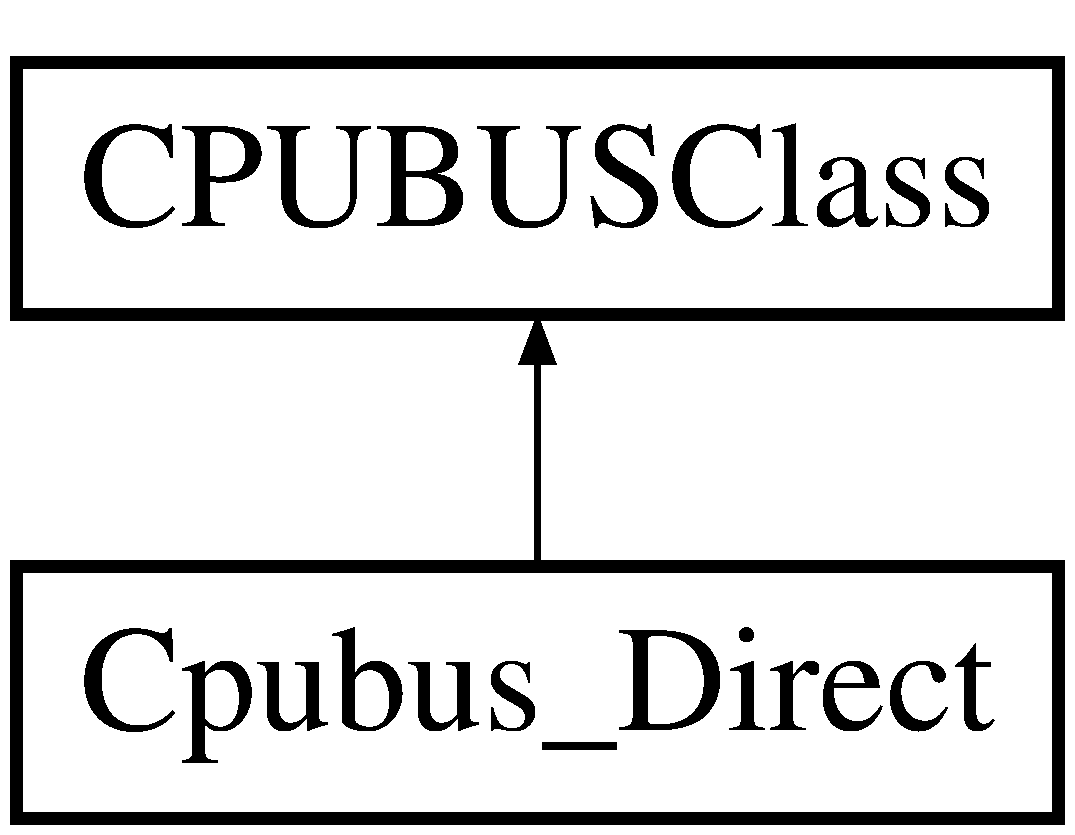
\includegraphics[height=2.000000cm]{classCpubus__Direct}
\end{center}
\end{figure}
\subsection*{Public Member Functions}
\begin{DoxyCompactItemize}
\item 
void \hyperlink{classCpubus__Direct_ac00959b9e99bacd23e89c1dbfc6d09a1}{init} (void)
\item 
uint8\-\_\-t \hyperlink{classCpubus__Direct_ad328ae744f1b2fc517d7344ac4306a3d}{read} (int address)
\item 
void \hyperlink{classCpubus__Direct_a3cdfb2389ddbccff39dcdde141377f99}{write} (int address, uint8\-\_\-t data)
\end{DoxyCompactItemize}


\subsection{Member Function Documentation}
\hypertarget{classCpubus__Direct_ac00959b9e99bacd23e89c1dbfc6d09a1}{\index{Cpubus\-\_\-\-Direct@{Cpubus\-\_\-\-Direct}!init@{init}}
\index{init@{init}!Cpubus_Direct@{Cpubus\-\_\-\-Direct}}
\subsubsection[{init}]{\setlength{\rightskip}{0pt plus 5cm}void Cpubus\-\_\-\-Direct\-::init (
\begin{DoxyParamCaption}
\item[{void}]{}
\end{DoxyParamCaption}
)\hspace{0.3cm}{\ttfamily [virtual]}}}\label{classCpubus__Direct_ac00959b9e99bacd23e89c1dbfc6d09a1}
Initialize the C\-P\-U\-B\-U\-S 

Reimplemented from \hyperlink{classCPUBUSClass_a1d678455708cddc708d36c099c107bce}{C\-P\-U\-B\-U\-S\-Class}.

\hypertarget{classCpubus__Direct_ad328ae744f1b2fc517d7344ac4306a3d}{\index{Cpubus\-\_\-\-Direct@{Cpubus\-\_\-\-Direct}!read@{read}}
\index{read@{read}!Cpubus_Direct@{Cpubus\-\_\-\-Direct}}
\subsubsection[{read}]{\setlength{\rightskip}{0pt plus 5cm}uint8\-\_\-t Cpubus\-\_\-\-Direct\-::read (
\begin{DoxyParamCaption}
\item[{int}]{address}
\end{DoxyParamCaption}
)\hspace{0.3cm}{\ttfamily [virtual]}}}\label{classCpubus__Direct_ad328ae744f1b2fc517d7344ac4306a3d}
read a byte from the C\-P\-U\-B\-U\-S 
\begin{DoxyParams}{Parameters}
{\em address} & 16bit address \\
\hline
\end{DoxyParams}
\begin{DoxyReturn}{Returns}
byte read from cpubus 
\end{DoxyReturn}


Reimplemented from \hyperlink{classCPUBUSClass_adaa8b8d537417bd7f372dbb8d575f783}{C\-P\-U\-B\-U\-S\-Class}.

\hypertarget{classCpubus__Direct_a3cdfb2389ddbccff39dcdde141377f99}{\index{Cpubus\-\_\-\-Direct@{Cpubus\-\_\-\-Direct}!write@{write}}
\index{write@{write}!Cpubus_Direct@{Cpubus\-\_\-\-Direct}}
\subsubsection[{write}]{\setlength{\rightskip}{0pt plus 5cm}void Cpubus\-\_\-\-Direct\-::write (
\begin{DoxyParamCaption}
\item[{int}]{address, }
\item[{uint8\-\_\-t}]{data}
\end{DoxyParamCaption}
)\hspace{0.3cm}{\ttfamily [virtual]}}}\label{classCpubus__Direct_a3cdfb2389ddbccff39dcdde141377f99}
write a byte from the C\-P\-U\-B\-U\-S 
\begin{DoxyParams}{Parameters}
{\em address} & 16 bit address \\
\hline
{\em byte} & to write \\
\hline
\end{DoxyParams}
\begin{DoxyReturn}{Returns}
none 
\end{DoxyReturn}


Reimplemented from \hyperlink{classCPUBUSClass_aafbcfc88bd0d0b7bf91010000e32fcf9}{C\-P\-U\-B\-U\-S\-Class}.



The documentation for this class was generated from the following files\-:\begin{DoxyCompactItemize}
\item 
\hyperlink{CPUBUS_8h}{C\-P\-U\-B\-U\-S.\-h}\item 
C\-P\-U\-B\-U\-S.\-cpp\end{DoxyCompactItemize}

\hypertarget{classCpubus__I2C}{\section{Cpubus\-\_\-\-I2\-C Class Reference}
\label{classCpubus__I2C}\index{Cpubus\-\_\-\-I2\-C@{Cpubus\-\_\-\-I2\-C}}
}
Inheritance diagram for Cpubus\-\_\-\-I2\-C\-:\begin{figure}[H]
\begin{center}
\leavevmode
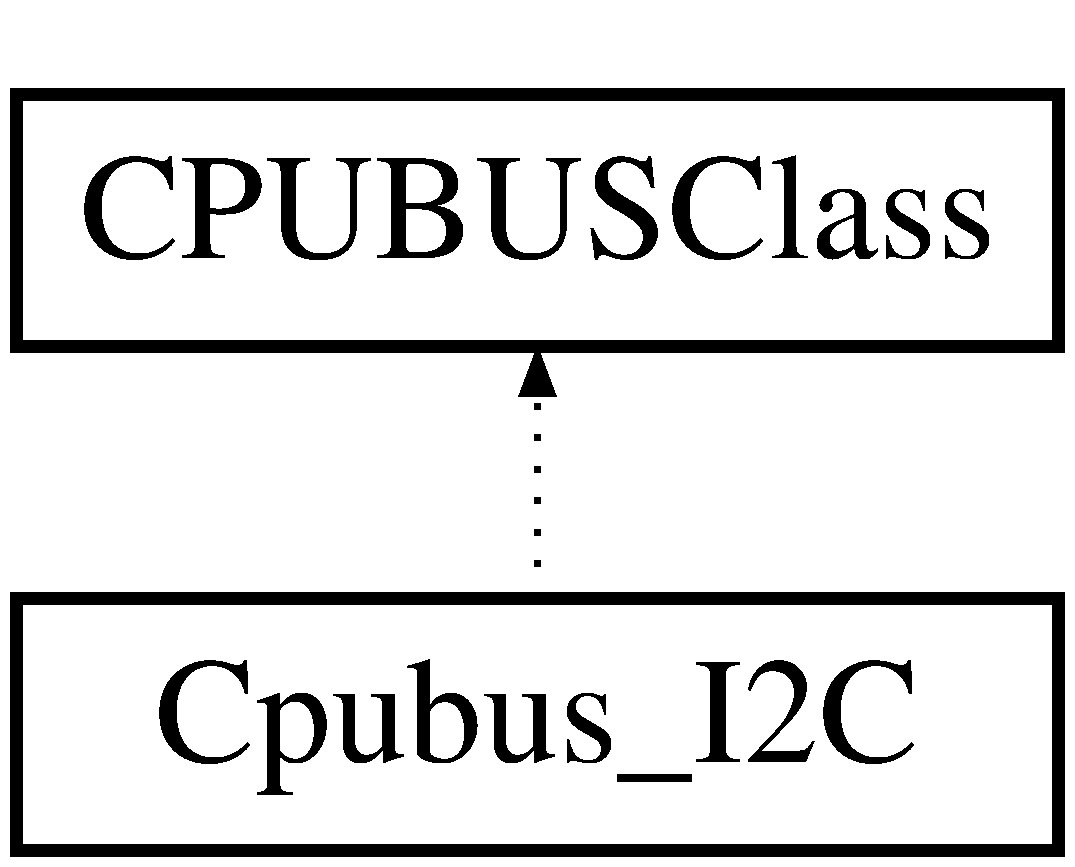
\includegraphics[height=2.000000cm]{classCpubus__I2C}
\end{center}
\end{figure}
\subsection*{Additional Inherited Members}


The documentation for this class was generated from the following file\-:\begin{DoxyCompactItemize}
\item 
\hyperlink{CPUBUS_8h}{C\-P\-U\-B\-U\-S.\-h}\end{DoxyCompactItemize}

\hypertarget{classCpubus__SPI}{\section{Cpubus\-\_\-\-S\-P\-I Class Reference}
\label{classCpubus__SPI}\index{Cpubus\-\_\-\-S\-P\-I@{Cpubus\-\_\-\-S\-P\-I}}
}
Inheritance diagram for Cpubus\-\_\-\-S\-P\-I\-:\begin{figure}[H]
\begin{center}
\leavevmode
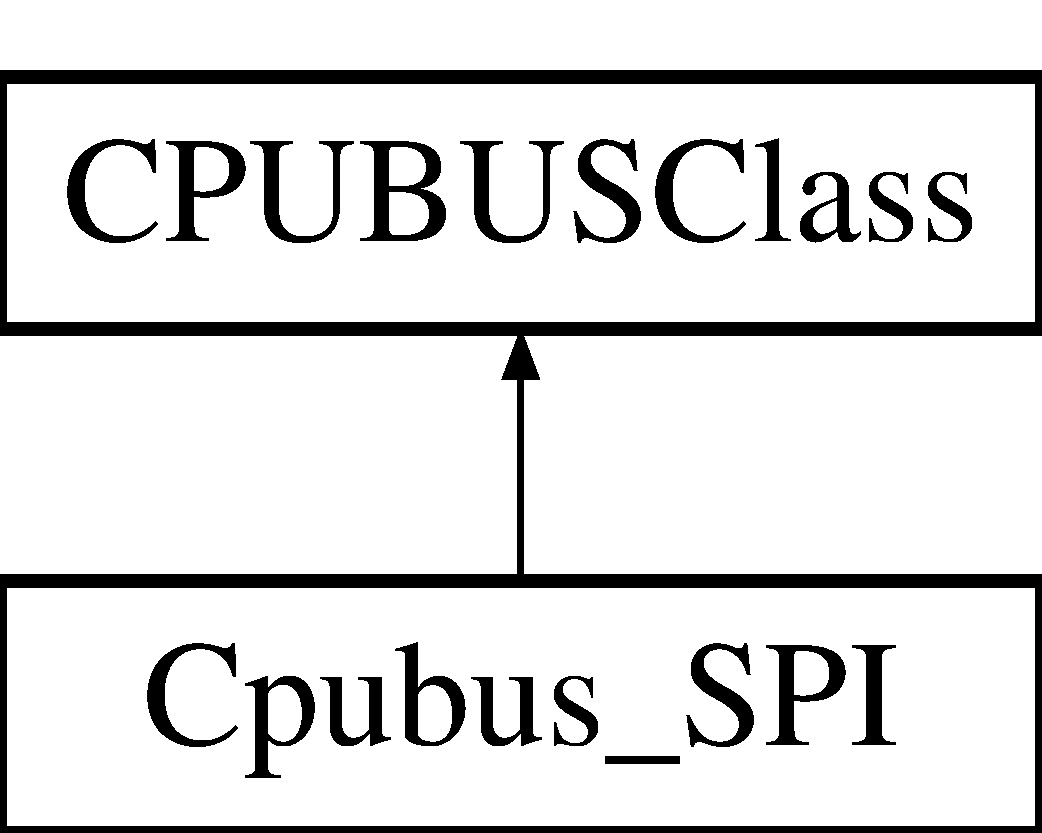
\includegraphics[height=2.000000cm]{classCpubus__SPI}
\end{center}
\end{figure}
\subsection*{Public Member Functions}
\begin{DoxyCompactItemize}
\item 
void \hyperlink{classCpubus__SPI_a0d95def08507883f4592f9ca96644263}{init} (void)
\item 
uint8\-\_\-t \hyperlink{classCpubus__SPI_a6710e52e4b221c1c999eecc30a73e676}{read} (int address)
\item 
void \hyperlink{classCpubus__SPI_a75d6b51bc35c93f1a0cfe56af86547b0}{write} (int address, uint8\-\_\-t data)
\end{DoxyCompactItemize}


\subsection{Member Function Documentation}
\hypertarget{classCpubus__SPI_a0d95def08507883f4592f9ca96644263}{\index{Cpubus\-\_\-\-S\-P\-I@{Cpubus\-\_\-\-S\-P\-I}!init@{init}}
\index{init@{init}!Cpubus_SPI@{Cpubus\-\_\-\-S\-P\-I}}
\subsubsection[{init}]{\setlength{\rightskip}{0pt plus 5cm}void Cpubus\-\_\-\-S\-P\-I\-::init (
\begin{DoxyParamCaption}
\item[{void}]{}
\end{DoxyParamCaption}
)\hspace{0.3cm}{\ttfamily [virtual]}}}\label{classCpubus__SPI_a0d95def08507883f4592f9ca96644263}
Initialize the C\-P\-U\-B\-U\-S 

Reimplemented from \hyperlink{classCPUBUSClass_a1d678455708cddc708d36c099c107bce}{C\-P\-U\-B\-U\-S\-Class}.

\hypertarget{classCpubus__SPI_a6710e52e4b221c1c999eecc30a73e676}{\index{Cpubus\-\_\-\-S\-P\-I@{Cpubus\-\_\-\-S\-P\-I}!read@{read}}
\index{read@{read}!Cpubus_SPI@{Cpubus\-\_\-\-S\-P\-I}}
\subsubsection[{read}]{\setlength{\rightskip}{0pt plus 5cm}uint8\-\_\-t Cpubus\-\_\-\-S\-P\-I\-::read (
\begin{DoxyParamCaption}
\item[{int}]{address}
\end{DoxyParamCaption}
)\hspace{0.3cm}{\ttfamily [virtual]}}}\label{classCpubus__SPI_a6710e52e4b221c1c999eecc30a73e676}
read a byte from the C\-P\-U\-B\-U\-S 
\begin{DoxyParams}{Parameters}
{\em address} & 16bit address \\
\hline
\end{DoxyParams}
\begin{DoxyReturn}{Returns}
byte read from cpubus 
\end{DoxyReturn}


Reimplemented from \hyperlink{classCPUBUSClass_adaa8b8d537417bd7f372dbb8d575f783}{C\-P\-U\-B\-U\-S\-Class}.

\hypertarget{classCpubus__SPI_a75d6b51bc35c93f1a0cfe56af86547b0}{\index{Cpubus\-\_\-\-S\-P\-I@{Cpubus\-\_\-\-S\-P\-I}!write@{write}}
\index{write@{write}!Cpubus_SPI@{Cpubus\-\_\-\-S\-P\-I}}
\subsubsection[{write}]{\setlength{\rightskip}{0pt plus 5cm}void Cpubus\-\_\-\-S\-P\-I\-::write (
\begin{DoxyParamCaption}
\item[{int}]{address, }
\item[{uint8\-\_\-t}]{data}
\end{DoxyParamCaption}
)\hspace{0.3cm}{\ttfamily [virtual]}}}\label{classCpubus__SPI_a75d6b51bc35c93f1a0cfe56af86547b0}
write a byte from the C\-P\-U\-B\-U\-S 
\begin{DoxyParams}{Parameters}
{\em address} & 16 bit address \\
\hline
{\em byte} & to write \\
\hline
\end{DoxyParams}
\begin{DoxyReturn}{Returns}
none 
\end{DoxyReturn}


Reimplemented from \hyperlink{classCPUBUSClass_aafbcfc88bd0d0b7bf91010000e32fcf9}{C\-P\-U\-B\-U\-S\-Class}.



The documentation for this class was generated from the following files\-:\begin{DoxyCompactItemize}
\item 
\hyperlink{CPUBUS_8h}{C\-P\-U\-B\-U\-S.\-h}\item 
C\-P\-U\-B\-U\-S.\-cpp\end{DoxyCompactItemize}

\hypertarget{classCPUBUSClass}{\section{C\-P\-U\-B\-U\-S\-Class Class Reference}
\label{classCPUBUSClass}\index{C\-P\-U\-B\-U\-S\-Class@{C\-P\-U\-B\-U\-S\-Class}}
}


{\ttfamily \#include $<$C\-P\-U\-B\-U\-S.\-h$>$}

Inheritance diagram for C\-P\-U\-B\-U\-S\-Class\-:\begin{figure}[H]
\begin{center}
\leavevmode
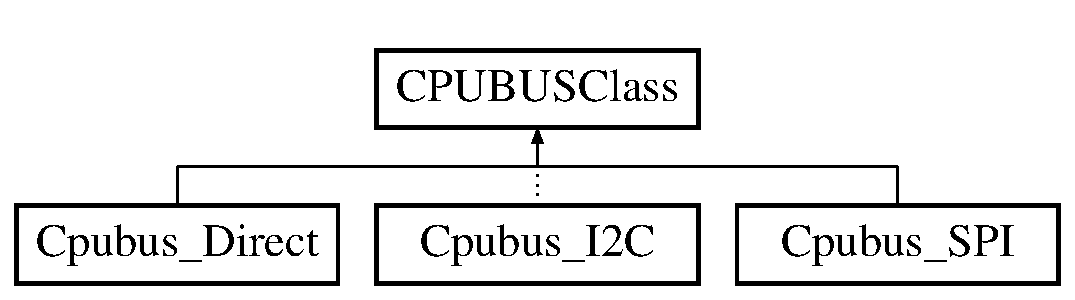
\includegraphics[height=2.000000cm]{classCPUBUSClass}
\end{center}
\end{figure}
\subsection*{Public Member Functions}
\begin{DoxyCompactItemize}
\item 
virtual void \hyperlink{classCPUBUSClass_a1d678455708cddc708d36c099c107bce}{init} (void)
\item 
virtual uint8\-\_\-t \hyperlink{classCPUBUSClass_adaa8b8d537417bd7f372dbb8d575f783}{read} (int address)
\item 
virtual void \hyperlink{classCPUBUSClass_aafbcfc88bd0d0b7bf91010000e32fcf9}{write} (int address, uint8\-\_\-t data)
\end{DoxyCompactItemize}


\subsection{Detailed Description}
This is the base class for C\-P\-U\-B\-U\-S, containing virtual functions 

\subsection{Member Function Documentation}
\hypertarget{classCPUBUSClass_a1d678455708cddc708d36c099c107bce}{\index{C\-P\-U\-B\-U\-S\-Class@{C\-P\-U\-B\-U\-S\-Class}!init@{init}}
\index{init@{init}!CPUBUSClass@{C\-P\-U\-B\-U\-S\-Class}}
\subsubsection[{init}]{\setlength{\rightskip}{0pt plus 5cm}virtual void C\-P\-U\-B\-U\-S\-Class\-::init (
\begin{DoxyParamCaption}
\item[{void}]{}
\end{DoxyParamCaption}
)\hspace{0.3cm}{\ttfamily [virtual]}}}\label{classCPUBUSClass_a1d678455708cddc708d36c099c107bce}
Initialize the C\-P\-U\-B\-U\-S 

Reimplemented in \hyperlink{classCpubus__SPI_a0d95def08507883f4592f9ca96644263}{Cpubus\-\_\-\-S\-P\-I}, and \hyperlink{classCpubus__Direct_ac00959b9e99bacd23e89c1dbfc6d09a1}{Cpubus\-\_\-\-Direct}.

\hypertarget{classCPUBUSClass_adaa8b8d537417bd7f372dbb8d575f783}{\index{C\-P\-U\-B\-U\-S\-Class@{C\-P\-U\-B\-U\-S\-Class}!read@{read}}
\index{read@{read}!CPUBUSClass@{C\-P\-U\-B\-U\-S\-Class}}
\subsubsection[{read}]{\setlength{\rightskip}{0pt plus 5cm}virtual uint8\-\_\-t C\-P\-U\-B\-U\-S\-Class\-::read (
\begin{DoxyParamCaption}
\item[{int}]{address}
\end{DoxyParamCaption}
)\hspace{0.3cm}{\ttfamily [virtual]}}}\label{classCPUBUSClass_adaa8b8d537417bd7f372dbb8d575f783}
read a byte from the C\-P\-U\-B\-U\-S 
\begin{DoxyParams}{Parameters}
{\em address} & 16bit address \\
\hline
\end{DoxyParams}
\begin{DoxyReturn}{Returns}
byte read from cpubus 
\end{DoxyReturn}


Reimplemented in \hyperlink{classCpubus__SPI_a6710e52e4b221c1c999eecc30a73e676}{Cpubus\-\_\-\-S\-P\-I}, and \hyperlink{classCpubus__Direct_ad328ae744f1b2fc517d7344ac4306a3d}{Cpubus\-\_\-\-Direct}.

\hypertarget{classCPUBUSClass_aafbcfc88bd0d0b7bf91010000e32fcf9}{\index{C\-P\-U\-B\-U\-S\-Class@{C\-P\-U\-B\-U\-S\-Class}!write@{write}}
\index{write@{write}!CPUBUSClass@{C\-P\-U\-B\-U\-S\-Class}}
\subsubsection[{write}]{\setlength{\rightskip}{0pt plus 5cm}virtual void C\-P\-U\-B\-U\-S\-Class\-::write (
\begin{DoxyParamCaption}
\item[{int}]{address, }
\item[{uint8\-\_\-t}]{data}
\end{DoxyParamCaption}
)\hspace{0.3cm}{\ttfamily [virtual]}}}\label{classCPUBUSClass_aafbcfc88bd0d0b7bf91010000e32fcf9}
write a byte from the C\-P\-U\-B\-U\-S 
\begin{DoxyParams}{Parameters}
{\em address} & 16 bit address \\
\hline
{\em byte} & to write \\
\hline
\end{DoxyParams}
\begin{DoxyReturn}{Returns}
none 
\end{DoxyReturn}


Reimplemented in \hyperlink{classCpubus__SPI_a75d6b51bc35c93f1a0cfe56af86547b0}{Cpubus\-\_\-\-S\-P\-I}, and \hyperlink{classCpubus__Direct_a3cdfb2389ddbccff39dcdde141377f99}{Cpubus\-\_\-\-Direct}.



The documentation for this class was generated from the following file\-:\begin{DoxyCompactItemize}
\item 
\hyperlink{CPUBUS_8h}{C\-P\-U\-B\-U\-S.\-h}\end{DoxyCompactItemize}

\hypertarget{classMC6821}{\section{M\-C6821 Class Reference}
\label{classMC6821}\index{M\-C6821@{M\-C6821}}
}
\subsection*{Public Member Functions}
\begin{DoxyCompactItemize}
\item 
\hypertarget{classMC6821_a6d0761549107b39339d5cf0dbbd7e8d6}{void {\bfseries init} (\hyperlink{classCPUBUSClass}{C\-P\-U\-B\-U\-S\-Class} $\ast$busptr, int addr)}\label{classMC6821_a6d0761549107b39339d5cf0dbbd7e8d6}

\item 
\hypertarget{classMC6821_adbe5f49d4668adc75086e868a9e61395}{uint8\-\_\-t {\bfseries read} (int address)}\label{classMC6821_adbe5f49d4668adc75086e868a9e61395}

\item 
\hypertarget{classMC6821_a0c93f2696f8d664d41920ffedca18451}{void {\bfseries write} (int address, uint8\-\_\-t data)}\label{classMC6821_a0c93f2696f8d664d41920ffedca18451}

\item 
\hypertarget{classMC6821_abc08642739f403a0e577e20709dd5cf7}{void {\bfseries write\-\_\-cra} (uint8\-\_\-t data)}\label{classMC6821_abc08642739f403a0e577e20709dd5cf7}

\item 
\hypertarget{classMC6821_a3a4cf42739e3051e0c1f7643a4a89c6e}{void {\bfseries write\-\_\-crb} (uint8\-\_\-t data)}\label{classMC6821_a3a4cf42739e3051e0c1f7643a4a89c6e}

\item 
\hypertarget{classMC6821_a9267b5d5a499a79f1cf67736475adbdf}{void {\bfseries write\-\_\-ddra} (uint8\-\_\-t data)}\label{classMC6821_a9267b5d5a499a79f1cf67736475adbdf}

\item 
\hypertarget{classMC6821_a6bb00a4e38b954182bb78a9a8388c11a}{void {\bfseries write\-\_\-ddrb} (uint8\-\_\-t data)}\label{classMC6821_a6bb00a4e38b954182bb78a9a8388c11a}

\item 
\hypertarget{classMC6821_a7d7766c34ae2f153ff2b31d4d472bdd9}{void {\bfseries write\-\_\-pdra} (uint8\-\_\-t data)}\label{classMC6821_a7d7766c34ae2f153ff2b31d4d472bdd9}

\item 
\hypertarget{classMC6821_a02885470c12c46c8145fb58057696283}{void {\bfseries write\-\_\-pdrb} (uint8\-\_\-t data)}\label{classMC6821_a02885470c12c46c8145fb58057696283}

\item 
\hypertarget{classMC6821_a17a8fd2101c222e02c56a23c11f192ad}{uint8\-\_\-t {\bfseries read\-\_\-pdra} ()}\label{classMC6821_a17a8fd2101c222e02c56a23c11f192ad}

\item 
\hypertarget{classMC6821_a4eb19034d534c7aa8b7d547234d1d8aa}{uint8\-\_\-t {\bfseries read\-\_\-pdrb} ()}\label{classMC6821_a4eb19034d534c7aa8b7d547234d1d8aa}

\item 
\hypertarget{classMC6821_a0e175c66f8a21c54bf2f1fa33ec1abf0}{uint8\-\_\-t {\bfseries read\-\_\-cra} ()}\label{classMC6821_a0e175c66f8a21c54bf2f1fa33ec1abf0}

\item 
\hypertarget{classMC6821_a0a03d067395eb7aa3a96fedc53fdc016}{uint8\-\_\-t {\bfseries read\-\_\-crb} ()}\label{classMC6821_a0a03d067395eb7aa3a96fedc53fdc016}

\item 
\hypertarget{classMC6821_a31a191a457f5de80cc172d89b50075c8}{void {\bfseries select\-\_\-ddra} ()}\label{classMC6821_a31a191a457f5de80cc172d89b50075c8}

\item 
\hypertarget{classMC6821_ae25d9cc7e1962fe822cfeef81df6d130}{void {\bfseries select\-\_\-ddrb} ()}\label{classMC6821_ae25d9cc7e1962fe822cfeef81df6d130}

\item 
\hypertarget{classMC6821_a2ffcdbd5b7756dd85c3eb09d5947391c}{void {\bfseries select\-\_\-pdra} ()}\label{classMC6821_a2ffcdbd5b7756dd85c3eb09d5947391c}

\item 
\hypertarget{classMC6821_a49928ce4a11ce0438545cb2e9d8aecc4}{void {\bfseries select\-\_\-pdrb} ()}\label{classMC6821_a49928ce4a11ce0438545cb2e9d8aecc4}

\end{DoxyCompactItemize}
\subsection*{Public Attributes}
\begin{DoxyCompactItemize}
\item 
\hypertarget{classMC6821_afc584e97eabf81051680b9a174bbce27}{\hyperlink{classCPUBUSClass}{C\-P\-U\-B\-U\-S\-Class} $\ast$ {\bfseries bus}}\label{classMC6821_afc584e97eabf81051680b9a174bbce27}

\item 
\hypertarget{classMC6821_afd059b6e851834c09f687e704f13c291}{int {\bfseries pia\-\_\-addr}}\label{classMC6821_afd059b6e851834c09f687e704f13c291}

\item 
\hypertarget{classMC6821_a620a47d50bb48aa7d3e1b7fc06606eb8}{int {\bfseries cra}}\label{classMC6821_a620a47d50bb48aa7d3e1b7fc06606eb8}

\item 
\hypertarget{classMC6821_a3b3c1610c32fc9c30cea82305bda9877}{int {\bfseries crb}}\label{classMC6821_a3b3c1610c32fc9c30cea82305bda9877}

\item 
\hypertarget{classMC6821_a9e4c3b0a432332a3171b7a64db5c9e2c}{int {\bfseries ddra}}\label{classMC6821_a9e4c3b0a432332a3171b7a64db5c9e2c}

\item 
\hypertarget{classMC6821_a3e4d74ba5f7a53d4df771a31153697f8}{int {\bfseries ddrb}}\label{classMC6821_a3e4d74ba5f7a53d4df771a31153697f8}

\item 
\hypertarget{classMC6821_abee44252a30363d98b5abcdd5745f9c0}{int {\bfseries pdra}}\label{classMC6821_abee44252a30363d98b5abcdd5745f9c0}

\item 
\hypertarget{classMC6821_ab8b937f3d2a6d17ae491261943376bd1}{int {\bfseries pdrb}}\label{classMC6821_ab8b937f3d2a6d17ae491261943376bd1}

\item 
\hypertarget{classMC6821_ad0dd3c7d0134188d0289b5df6223efce}{uint8\-\_\-t {\bfseries cra\-\_\-sv}}\label{classMC6821_ad0dd3c7d0134188d0289b5df6223efce}

\item 
\hypertarget{classMC6821_a93a9efc2dc448b508e944f4534565b53}{uint8\-\_\-t {\bfseries crb\-\_\-sv}}\label{classMC6821_a93a9efc2dc448b508e944f4534565b53}

\item 
\hypertarget{classMC6821_a1cf9d17cbc77627cc6610f72c0eb404b}{uint8\-\_\-t {\bfseries ddra\-\_\-sv}}\label{classMC6821_a1cf9d17cbc77627cc6610f72c0eb404b}

\item 
\hypertarget{classMC6821_a4d2ff521e77c816523f5a49d11a016bc}{uint8\-\_\-t {\bfseries ddrb\-\_\-sv}}\label{classMC6821_a4d2ff521e77c816523f5a49d11a016bc}

\item 
\hypertarget{classMC6821_ac85538eaa73e200b018baa5a12f5925e}{uint8\-\_\-t {\bfseries pdra\-\_\-sv}}\label{classMC6821_ac85538eaa73e200b018baa5a12f5925e}

\item 
\hypertarget{classMC6821_a3c588f5962575cb9ea95995aa770b7e3}{uint8\-\_\-t {\bfseries pdrb\-\_\-sv}}\label{classMC6821_a3c588f5962575cb9ea95995aa770b7e3}

\end{DoxyCompactItemize}


The documentation for this class was generated from the following files\-:\begin{DoxyCompactItemize}
\item 
mc6821.\-h\item 
mc6821.\-cpp\end{DoxyCompactItemize}

\hypertarget{classMCP23S17}{\section{M\-C\-P23\-S17 Class Reference}
\label{classMCP23S17}\index{M\-C\-P23\-S17@{M\-C\-P23\-S17}}
}
\subsection*{Public Member Functions}
\begin{DoxyCompactItemize}
\item 
\hypertarget{classMCP23S17_a47e81be4746f042f8cf3e8c6c58ad9f8}{{\bfseries M\-C\-P23\-S17} (uint8\-\_\-t slave\-\_\-select)}\label{classMCP23S17_a47e81be4746f042f8cf3e8c6c58ad9f8}

\item 
\hypertarget{classMCP23S17_ab9c8589b93f55157d435265225adec41}{{\bfseries M\-C\-P23\-S17} (uint8\-\_\-t slave\-\_\-select, byte aaa\-\_\-hw\-\_\-addr)}\label{classMCP23S17_ab9c8589b93f55157d435265225adec41}

\item 
\hypertarget{classMCP23S17_a5ee683f0730a23417ecee5bf9c812ea1}{void {\bfseries pin\-Mode} (bool mode)}\label{classMCP23S17_a5ee683f0730a23417ecee5bf9c812ea1}

\item 
\hypertarget{classMCP23S17_a6e0f45191fd20c584f4e8780ba3d75c5}{void {\bfseries port} (uint16\-\_\-t value)}\label{classMCP23S17_a6e0f45191fd20c584f4e8780ba3d75c5}

\item 
\hypertarget{classMCP23S17_a4dac8c3835c31757b951a693d89aa14d}{uint16\-\_\-t {\bfseries port} ()}\label{classMCP23S17_a4dac8c3835c31757b951a693d89aa14d}

\item 
\hypertarget{classMCP23S17_a58044c38e93ac371e3a1697d6bc6265f}{void {\bfseries pin\-Mode} (uint8\-\_\-t pin, bool mode)}\label{classMCP23S17_a58044c38e93ac371e3a1697d6bc6265f}

\item 
\hypertarget{classMCP23S17_ae5a682bcd30f962bc7b40531d568441a}{void {\bfseries digital\-Write} (uint8\-\_\-t pin, bool value)}\label{classMCP23S17_ae5a682bcd30f962bc7b40531d568441a}

\item 
\hypertarget{classMCP23S17_a09738975e423ab784c8ea46b24ea0109}{int {\bfseries digital\-Read} (uint8\-\_\-t pin)}\label{classMCP23S17_a09738975e423ab784c8ea46b24ea0109}

\end{DoxyCompactItemize}
\subsection*{Static Public Attributes}
\begin{DoxyCompactItemize}
\item 
\hypertarget{classMCP23S17_a759ef1c2480227759d5b5ea05ffecce0}{static const uint8\-\_\-t {\bfseries G\-P\-I\-O\-\_\-\-A0} = 0}\label{classMCP23S17_a759ef1c2480227759d5b5ea05ffecce0}

\item 
\hypertarget{classMCP23S17_a334689a00aeeae7947eaff662dee942a}{static const uint8\-\_\-t {\bfseries G\-P\-I\-O\-\_\-\-A1} = 1}\label{classMCP23S17_a334689a00aeeae7947eaff662dee942a}

\item 
\hypertarget{classMCP23S17_ab1ee881157292443cbf8eb0f33d1418b}{static const uint8\-\_\-t {\bfseries G\-P\-I\-O\-\_\-\-A2} = 2}\label{classMCP23S17_ab1ee881157292443cbf8eb0f33d1418b}

\item 
\hypertarget{classMCP23S17_a16df8b0338dd0568ee7bf4683ce8b1fd}{static const uint8\-\_\-t {\bfseries G\-P\-I\-O\-\_\-\-A3} = 3}\label{classMCP23S17_a16df8b0338dd0568ee7bf4683ce8b1fd}

\item 
\hypertarget{classMCP23S17_a9b8d7dd871b10ad7100d39e5b2267bc7}{static const uint8\-\_\-t {\bfseries G\-P\-I\-O\-\_\-\-A4} = 4}\label{classMCP23S17_a9b8d7dd871b10ad7100d39e5b2267bc7}

\item 
\hypertarget{classMCP23S17_a28af569b31d638738a26c42de4d17ea0}{static const uint8\-\_\-t {\bfseries G\-P\-I\-O\-\_\-\-A5} = 5}\label{classMCP23S17_a28af569b31d638738a26c42de4d17ea0}

\item 
\hypertarget{classMCP23S17_ae3d3c04d465f7a876adbe2857f2858be}{static const uint8\-\_\-t {\bfseries G\-P\-I\-O\-\_\-\-A6} = 6}\label{classMCP23S17_ae3d3c04d465f7a876adbe2857f2858be}

\item 
\hypertarget{classMCP23S17_a7bd98b1d3749547b98b40580fe019f54}{static const uint8\-\_\-t {\bfseries G\-P\-I\-O\-\_\-\-A7} = 7}\label{classMCP23S17_a7bd98b1d3749547b98b40580fe019f54}

\item 
\hypertarget{classMCP23S17_af6f1bce620edac01e8dfdca481e32699}{static const uint8\-\_\-t {\bfseries G\-P\-I\-O\-\_\-\-B0} = 8}\label{classMCP23S17_af6f1bce620edac01e8dfdca481e32699}

\item 
\hypertarget{classMCP23S17_aaab9326a3b175bdeb3688065c2cc1a94}{static const uint8\-\_\-t {\bfseries G\-P\-I\-O\-\_\-\-B1} = 9}\label{classMCP23S17_aaab9326a3b175bdeb3688065c2cc1a94}

\item 
\hypertarget{classMCP23S17_a0b7a1e4079576c231ae2e5395099b725}{static const uint8\-\_\-t {\bfseries G\-P\-I\-O\-\_\-\-B2} = 10}\label{classMCP23S17_a0b7a1e4079576c231ae2e5395099b725}

\item 
\hypertarget{classMCP23S17_a418a13cbefcdae5b3f3f263644280050}{static const uint8\-\_\-t {\bfseries G\-P\-I\-O\-\_\-\-B3} = 11}\label{classMCP23S17_a418a13cbefcdae5b3f3f263644280050}

\item 
\hypertarget{classMCP23S17_af24167b51de8e80d830eae869c013698}{static const uint8\-\_\-t {\bfseries G\-P\-I\-O\-\_\-\-B4} = 12}\label{classMCP23S17_af24167b51de8e80d830eae869c013698}

\item 
\hypertarget{classMCP23S17_a48da719a328d3e91ae944cdbc80ff142}{static const uint8\-\_\-t {\bfseries G\-P\-I\-O\-\_\-\-B5} = 13}\label{classMCP23S17_a48da719a328d3e91ae944cdbc80ff142}

\item 
\hypertarget{classMCP23S17_a331b53631d93700508fe83c6716d506a}{static const uint8\-\_\-t {\bfseries G\-P\-I\-O\-\_\-\-B6} = 14}\label{classMCP23S17_a331b53631d93700508fe83c6716d506a}

\item 
\hypertarget{classMCP23S17_ace3c345f331da5f48fc2cb7df69d1591}{static const uint8\-\_\-t {\bfseries G\-P\-I\-O\-\_\-\-B7} = 15}\label{classMCP23S17_ace3c345f331da5f48fc2cb7df69d1591}

\end{DoxyCompactItemize}
\subsection*{Protected Member Functions}
\begin{DoxyCompactItemize}
\item 
\hypertarget{classMCP23S17_adc533f57a1c273a561ba8c43ef16583b}{void {\bfseries setup\-\_\-ss} (uint8\-\_\-t slave\-\_\-select\-\_\-pin)}\label{classMCP23S17_adc533f57a1c273a561ba8c43ef16583b}

\item 
\hypertarget{classMCP23S17_abfe8b764df74c1cd67d6f80abed9779a}{void {\bfseries setup\-\_\-device} (uint8\-\_\-t aaa\-\_\-hw\-\_\-addr)}\label{classMCP23S17_abfe8b764df74c1cd67d6f80abed9779a}

\item 
\hypertarget{classMCP23S17_acca0ab791c54a6ac93d1b54c94418ab5}{uint16\-\_\-t {\bfseries read\-\_\-addr} (byte addr)}\label{classMCP23S17_acca0ab791c54a6ac93d1b54c94418ab5}

\item 
\hypertarget{classMCP23S17_a318f98c1869e89485dcf3d2e1d994733}{void {\bfseries write\-\_\-addr} (byte addr, uint16\-\_\-t data)}\label{classMCP23S17_a318f98c1869e89485dcf3d2e1d994733}

\item 
\hypertarget{classMCP23S17_a7d9564ada8cedac7b6af214f79d172f2}{void {\bfseries write\-\_\-addr\-\_\-byte} (byte addr, uint8\-\_\-t data)}\label{classMCP23S17_a7d9564ada8cedac7b6af214f79d172f2}

\item 
\hypertarget{classMCP23S17_a6a6994827805f68850486de7ddd8ff56}{uint16\-\_\-t {\bfseries byte2uint16} (byte high\-\_\-byte, byte low\-\_\-byte)}\label{classMCP23S17_a6a6994827805f68850486de7ddd8ff56}

\item 
\hypertarget{classMCP23S17_a14ae844e7dac5033a13ce67cadb21864}{byte {\bfseries uint16\-\_\-high\-\_\-byte} (uint16\-\_\-t uint16)}\label{classMCP23S17_a14ae844e7dac5033a13ce67cadb21864}

\item 
\hypertarget{classMCP23S17_a5cf7aba638399ec9b4883079ae44dc35}{byte {\bfseries uint16\-\_\-low\-\_\-byte} (uint16\-\_\-t uint16)}\label{classMCP23S17_a5cf7aba638399ec9b4883079ae44dc35}

\end{DoxyCompactItemize}
\subsection*{Protected Attributes}
\begin{DoxyCompactItemize}
\item 
\hypertarget{classMCP23S17_a4dd9535162684571fe934fd26b3f5531}{uint8\-\_\-t {\bfseries slave\-\_\-select\-\_\-pin}}\label{classMCP23S17_a4dd9535162684571fe934fd26b3f5531}

\item 
\hypertarget{classMCP23S17_a6ee55dd507b28ccb620810cf40c1d681}{byte {\bfseries aaa\-\_\-hw\-\_\-addr}}\label{classMCP23S17_a6ee55dd507b28ccb620810cf40c1d681}

\item 
\hypertarget{classMCP23S17_a1a21ef06797ed6899ab8f86087a90389}{byte {\bfseries read\-\_\-cmd}}\label{classMCP23S17_a1a21ef06797ed6899ab8f86087a90389}

\item 
\hypertarget{classMCP23S17_ad9c64890ebb6e80306fdb070578782c0}{byte {\bfseries write\-\_\-cmd}}\label{classMCP23S17_ad9c64890ebb6e80306fdb070578782c0}

\end{DoxyCompactItemize}
\subsection*{Static Protected Attributes}
\begin{DoxyCompactItemize}
\item 
\hypertarget{classMCP23S17_abbe37643146bb9195797ffda7f43d66f}{static const uint8\-\_\-t {\bfseries I\-O\-C\-O\-N\-A} = 0x0\-A}\label{classMCP23S17_abbe37643146bb9195797ffda7f43d66f}

\item 
\hypertarget{classMCP23S17_a63859159568a5837034bb88b20c53e2d}{static const uint8\-\_\-t {\bfseries I\-O\-C\-O\-N} = I\-O\-C\-O\-N\-A}\label{classMCP23S17_a63859159568a5837034bb88b20c53e2d}

\item 
\hypertarget{classMCP23S17_a19eebedb9b1a7c2a572245b78b93d8dc}{static const uint8\-\_\-t {\bfseries S\-E\-Q\-O\-P} = 0b00100000}\label{classMCP23S17_a19eebedb9b1a7c2a572245b78b93d8dc}

\item 
\hypertarget{classMCP23S17_a599afe026032676b92035a8988750c60}{static const uint8\-\_\-t {\bfseries H\-A\-E\-N} = 0b00001000}\label{classMCP23S17_a599afe026032676b92035a8988750c60}

\item 
\hypertarget{classMCP23S17_a1c8011f21ae71b1bb9c0f2da7b3bb1be}{static const uint8\-\_\-t {\bfseries I\-O\-D\-I\-R\-A} = 0x00}\label{classMCP23S17_a1c8011f21ae71b1bb9c0f2da7b3bb1be}

\item 
\hypertarget{classMCP23S17_a54be44f7e7d58f8cd4c2876e92b1bc39}{static const uint8\-\_\-t {\bfseries I\-O\-D\-I\-R\-B} = 0x01}\label{classMCP23S17_a54be44f7e7d58f8cd4c2876e92b1bc39}

\item 
\hypertarget{classMCP23S17_af9d4a7f36be2498e9fa443af2341d2d7}{static const uint8\-\_\-t {\bfseries I\-O\-D\-I\-R} = I\-O\-D\-I\-R\-A}\label{classMCP23S17_af9d4a7f36be2498e9fa443af2341d2d7}

\item 
\hypertarget{classMCP23S17_a1eefc3383b32c26f17dfe9709b3f8e7c}{static const uint8\-\_\-t {\bfseries G\-P\-P\-U\-A} = 0x0\-C}\label{classMCP23S17_a1eefc3383b32c26f17dfe9709b3f8e7c}

\item 
\hypertarget{classMCP23S17_aa627e5b8b5fb31f810446b7383683a49}{static const uint8\-\_\-t {\bfseries G\-P\-P\-U\-B} = 0x0\-D}\label{classMCP23S17_aa627e5b8b5fb31f810446b7383683a49}

\item 
\hypertarget{classMCP23S17_ae33660d68c052be00398ce25eddda821}{static const uint8\-\_\-t {\bfseries G\-P\-P\-U} = G\-P\-P\-U\-A}\label{classMCP23S17_ae33660d68c052be00398ce25eddda821}

\item 
\hypertarget{classMCP23S17_a35c11ee2e9c47694f0282d4f88454be8}{static const uint8\-\_\-t {\bfseries G\-P\-I\-O\-A} = 0x12}\label{classMCP23S17_a35c11ee2e9c47694f0282d4f88454be8}

\item 
\hypertarget{classMCP23S17_a7384014fa658f34e3a22260a202f15cc}{static const uint8\-\_\-t {\bfseries G\-P\-I\-O\-B} = 0x13}\label{classMCP23S17_a7384014fa658f34e3a22260a202f15cc}

\item 
\hypertarget{classMCP23S17_ab9813abef800a5f2c1b9acb74ef56c53}{static const uint8\-\_\-t {\bfseries G\-P\-I\-O} = G\-P\-I\-O\-A}\label{classMCP23S17_ab9813abef800a5f2c1b9acb74ef56c53}

\end{DoxyCompactItemize}


The documentation for this class was generated from the following files\-:\begin{DoxyCompactItemize}
\item 
Mcp23s17.\-h\item 
Mcp23s17.\-cpp\end{DoxyCompactItemize}

\hypertarget{classROM}{\section{R\-O\-M Class Reference}
\label{classROM}\index{R\-O\-M@{R\-O\-M}}
}
\subsection*{Public Member Functions}
\begin{DoxyCompactItemize}
\item 
\hypertarget{classROM_aea2555cada1d077a6dfaf96380fc1fc0}{void {\bfseries init} (\hyperlink{classCPUBUSClass}{C\-P\-U\-B\-U\-S\-Class} $\ast$busptr, int addr, int size)}\label{classROM_aea2555cada1d077a6dfaf96380fc1fc0}

\item 
\hypertarget{classROM_ac3bb73826a151ceda7c80fe1e4f45331}{uint8\-\_\-t {\bfseries read} (int address)}\label{classROM_ac3bb73826a151ceda7c80fe1e4f45331}

\item 
\hypertarget{classROM_a6b9d004b23b2ba9d65eb9de41b75d250}{uint8\-\_\-t {\bfseries read\-\_\-offset} (int address)}\label{classROM_a6b9d004b23b2ba9d65eb9de41b75d250}

\item 
\hypertarget{classROM_afccfd3650bbd6ed1637f5ead844e86a1}{void {\bfseries dump} ()}\label{classROM_afccfd3650bbd6ed1637f5ead844e86a1}

\end{DoxyCompactItemize}
\subsection*{Public Attributes}
\begin{DoxyCompactItemize}
\item 
\hypertarget{classROM_aa0e8713b59fee793cd51f8657342242b}{\hyperlink{classCPUBUSClass}{C\-P\-U\-B\-U\-S\-Class} $\ast$ {\bfseries bus}}\label{classROM_aa0e8713b59fee793cd51f8657342242b}

\item 
\hypertarget{classROM_a88a16bc3dcf8e2c2b9e056eca070994e}{int {\bfseries rom\-\_\-address}}\label{classROM_a88a16bc3dcf8e2c2b9e056eca070994e}

\item 
\hypertarget{classROM_ab088631203d67cb90eb7711b64c2ac32}{int {\bfseries rom\-\_\-size}}\label{classROM_ab088631203d67cb90eb7711b64c2ac32}

\end{DoxyCompactItemize}


The documentation for this class was generated from the following files\-:\begin{DoxyCompactItemize}
\item 
rom.\-h\item 
rom.\-cpp\end{DoxyCompactItemize}

\chapter{File Documentation}
\hypertarget{CPUBUS_8h}{\section{C\-P\-U\-B\-U\-S.\-h File Reference}
\label{CPUBUS_8h}\index{C\-P\-U\-B\-U\-S.\-h@{C\-P\-U\-B\-U\-S.\-h}}
}


Classes to use the address/data bus.  


{\ttfamily \#include $<$inttypes.\-h$>$}\\*
{\ttfamily \#include $<$S\-P\-I.\-h$>$}\\*
{\ttfamily \#include \char`\"{}Mcp23s17.\-h\char`\"{}}\\*
{\ttfamily \#include \char`\"{}W\-Program.\-h\char`\"{}}\\*
\subsection*{Classes}
\begin{DoxyCompactItemize}
\item 
class \hyperlink{classCPUBUSClass}{C\-P\-U\-B\-U\-S\-Class}
\item 
class \hyperlink{classCpubus__Direct}{Cpubus\-\_\-\-Direct}
\item 
class \hyperlink{classCpubus__SPI}{Cpubus\-\_\-\-S\-P\-I}
\item 
class \hyperlink{classCpubus__I2C}{Cpubus\-\_\-\-I2\-C}
\end{DoxyCompactItemize}
\subsection*{Macros}
\begin{DoxyCompactItemize}
\item 
\hypertarget{CPUBUS_8h_a8751c246556128a9c81cb083679c2d88}{\#define {\bfseries C\-P\-U\-B\-U\-S\-\_\-\-D\-I\-R\-E\-C\-T}~0}\label{CPUBUS_8h_a8751c246556128a9c81cb083679c2d88}

\item 
\hypertarget{CPUBUS_8h_a27c0ce38d6527788c5433b5f7c7f1b78}{\#define {\bfseries C\-P\-U\-B\-U\-S\-\_\-\-S\-P\-I}~1}\label{CPUBUS_8h_a27c0ce38d6527788c5433b5f7c7f1b78}

\item 
\hypertarget{CPUBUS_8h_abb1a2686513890b5857e526657860455}{\#define {\bfseries C\-P\-U\-B\-U\-S\-\_\-\-I2\-C}~2}\label{CPUBUS_8h_abb1a2686513890b5857e526657860455}

\item 
\hypertarget{CPUBUS_8h_ae6567cddde2bd0d56e67f39b014c0513}{\#define {\bfseries C\-P\-U\-B\-U\-S\-\_\-\-D\-A\-T\-A\-\_\-\-P\-O\-R\-T}~P\-O\-R\-T\-L}\label{CPUBUS_8h_ae6567cddde2bd0d56e67f39b014c0513}

\item 
\hypertarget{CPUBUS_8h_a32ac3149462201e445940fadcae025e3}{\#define {\bfseries C\-P\-U\-B\-U\-S\-\_\-\-D\-A\-T\-A\-\_\-\-P\-I\-N\-S}~P\-I\-N\-L}\label{CPUBUS_8h_a32ac3149462201e445940fadcae025e3}

\item 
\hypertarget{CPUBUS_8h_a53c0ae1c185f7724ff1d93019f684cb0}{\#define {\bfseries C\-P\-U\-B\-U\-S\-\_\-\-D\-A\-T\-A\-\_\-\-D\-D\-R}~D\-D\-R\-L}\label{CPUBUS_8h_a53c0ae1c185f7724ff1d93019f684cb0}

\item 
\hypertarget{CPUBUS_8h_a7bfe5de717a3b1cee34159d48cd0173e}{\#define {\bfseries C\-P\-U\-B\-U\-S\-\_\-\-A\-D\-D\-R\-L\-\_\-\-P\-O\-R\-T}~P\-O\-R\-T\-A}\label{CPUBUS_8h_a7bfe5de717a3b1cee34159d48cd0173e}

\item 
\hypertarget{CPUBUS_8h_ac3e83440fa39ef12216c23a8c7898713}{\#define {\bfseries C\-P\-U\-B\-U\-S\-\_\-\-A\-D\-D\-R\-L\-\_\-\-P\-I\-N\-S}~P\-I\-N\-A}\label{CPUBUS_8h_ac3e83440fa39ef12216c23a8c7898713}

\item 
\hypertarget{CPUBUS_8h_ae3f4dd64ae2c9502e0e1dcbd39f52213}{\#define {\bfseries C\-P\-U\-B\-U\-S\-\_\-\-A\-D\-D\-R\-L\-\_\-\-D\-D\-R}~D\-D\-R\-A}\label{CPUBUS_8h_ae3f4dd64ae2c9502e0e1dcbd39f52213}

\item 
\hypertarget{CPUBUS_8h_aff0f1da72741651958286469ee31b586}{\#define {\bfseries C\-P\-U\-B\-U\-S\-\_\-\-A\-D\-D\-R\-H\-\_\-\-P\-O\-R\-T}~P\-O\-R\-T\-C}\label{CPUBUS_8h_aff0f1da72741651958286469ee31b586}

\item 
\hypertarget{CPUBUS_8h_a173e4b6f334d48d1e0be40288c189792}{\#define {\bfseries C\-P\-U\-B\-U\-S\-\_\-\-A\-D\-D\-R\-H\-\_\-\-P\-I\-N\-S}~P\-I\-N\-C}\label{CPUBUS_8h_a173e4b6f334d48d1e0be40288c189792}

\item 
\hypertarget{CPUBUS_8h_ac6b5dcd7b8a02585dc6c9db48effa6de}{\#define {\bfseries C\-P\-U\-B\-U\-S\-\_\-\-A\-D\-D\-R\-H\-\_\-\-D\-D\-R}~D\-D\-R\-C}\label{CPUBUS_8h_ac6b5dcd7b8a02585dc6c9db48effa6de}

\item 
\hypertarget{CPUBUS_8h_a7c8fe1bdcb8febd9808589f2f7436cd5}{\#define {\bfseries C\-P\-U\-B\-U\-S\-\_\-\-C\-T\-L\-\_\-\-P\-O\-R\-T}~P\-O\-R\-T\-F}\label{CPUBUS_8h_a7c8fe1bdcb8febd9808589f2f7436cd5}

\item 
\hypertarget{CPUBUS_8h_aaee9ce5f08890f61bb7dab948a3ae0f9}{\#define {\bfseries C\-P\-U\-B\-U\-S\-\_\-\-C\-T\-L\-\_\-\-P\-I\-N\-S}~P\-I\-N\-F}\label{CPUBUS_8h_aaee9ce5f08890f61bb7dab948a3ae0f9}

\item 
\hypertarget{CPUBUS_8h_aadeba9b013b14630f94f3cc4404aff69}{\#define {\bfseries C\-P\-U\-B\-U\-S\-\_\-\-C\-T\-L\-\_\-\-D\-D\-R}~D\-D\-R\-F}\label{CPUBUS_8h_aadeba9b013b14630f94f3cc4404aff69}

\item 
\hypertarget{CPUBUS_8h_add70edb506f10bd2b156e19bb3c754fa}{\#define {\bfseries C\-P\-U\-B\-U\-S\-\_\-\-R\-W}~0}\label{CPUBUS_8h_add70edb506f10bd2b156e19bb3c754fa}

\item 
\hypertarget{CPUBUS_8h_a035f625f8dbdbdcc800ba0d887e4bbce}{\#define {\bfseries C\-P\-U\-B\-U\-S\-\_\-\-E}~1}\label{CPUBUS_8h_a035f625f8dbdbdcc800ba0d887e4bbce}

\item 
\hypertarget{CPUBUS_8h_a33468c9d433b3596a23ab44eeff547c8}{\#define {\bfseries C\-P\-U\-B\-U\-S\-\_\-\-V\-M\-A}~2}\label{CPUBUS_8h_a33468c9d433b3596a23ab44eeff547c8}

\item 
\hypertarget{CPUBUS_8h_a0bdf0e5205ae19fad781b1a72af788f9}{\#define {\bfseries C\-P\-U\-B\-U\-S\-\_\-\-R\-E\-S\-E\-T}~3}\label{CPUBUS_8h_a0bdf0e5205ae19fad781b1a72af788f9}

\item 
\hypertarget{CPUBUS_8h_a080163c5331814a7fabe11a5bd248b84}{\#define {\bfseries C\-P\-U\-B\-U\-S\-\_\-\-H\-A\-L\-T}~4}\label{CPUBUS_8h_a080163c5331814a7fabe11a5bd248b84}

\item 
\hypertarget{CPUBUS_8h_abd84c98f29d44d5fdf933f5cc635e62b}{\#define {\bfseries C\-P\-U\-B\-U\-S\-\_\-\-M\-R}~5}\label{CPUBUS_8h_abd84c98f29d44d5fdf933f5cc635e62b}

\item 
\hypertarget{CPUBUS_8h_a86770688ff2aa4db3e939cc8068cc8b6}{\#define {\bfseries C\-P\-U\-B\-U\-S\-\_\-\-I\-R\-Q}~6}\label{CPUBUS_8h_a86770688ff2aa4db3e939cc8068cc8b6}

\item 
\hypertarget{CPUBUS_8h_a6bfc5918f33c30af4322f8e7888206af}{\#define {\bfseries C\-P\-U\-B\-U\-S\-\_\-\-N\-M\-I}~7}\label{CPUBUS_8h_a6bfc5918f33c30af4322f8e7888206af}

\item 
\hypertarget{CPUBUS_8h_a59c9067a171de84235eebf31259466ca}{\#define {\bfseries C\-P\-U\-B\-U\-S\-\_\-\-R\-W\-\_\-\-P\-I\-N}~A0}\label{CPUBUS_8h_a59c9067a171de84235eebf31259466ca}

\item 
\hypertarget{CPUBUS_8h_a4d12372996090c9ce3496307f1b58da4}{\#define {\bfseries C\-P\-U\-B\-U\-S\-\_\-\-E\-\_\-\-P\-I\-N}~A1}\label{CPUBUS_8h_a4d12372996090c9ce3496307f1b58da4}

\item 
\hypertarget{CPUBUS_8h_a568ab109696e8c25258f8626f914ee0b}{\#define {\bfseries C\-P\-U\-B\-U\-S\-\_\-\-V\-M\-A\-\_\-\-P\-I\-N}~A2}\label{CPUBUS_8h_a568ab109696e8c25258f8626f914ee0b}

\item 
\hypertarget{CPUBUS_8h_af47271afc3de50255dc7ca87ee1cdda5}{\#define {\bfseries C\-P\-U\-B\-U\-S\-\_\-\-R\-E\-S\-E\-T\-\_\-\-P\-I\-N}~A3}\label{CPUBUS_8h_af47271afc3de50255dc7ca87ee1cdda5}

\item 
\hypertarget{CPUBUS_8h_af4065a8fb4331dcddecc617dc4f0b5f9}{\#define {\bfseries C\-P\-U\-B\-U\-S\-\_\-\-H\-A\-L\-T\-\_\-\-P\-I\-N}~A4}\label{CPUBUS_8h_af4065a8fb4331dcddecc617dc4f0b5f9}

\item 
\hypertarget{CPUBUS_8h_abb9e7a5eb182a8c2ed4d58d258cd782e}{\#define {\bfseries C\-P\-U\-B\-U\-S\-\_\-\-M\-R\-\_\-\-P\-I\-N}~A5}\label{CPUBUS_8h_abb9e7a5eb182a8c2ed4d58d258cd782e}

\item 
\hypertarget{CPUBUS_8h_a4a192b83d6d2c65320436790fccf1cef}{\#define {\bfseries C\-P\-U\-B\-U\-S\-\_\-\-I\-R\-Q\-\_\-\-P\-I\-N}~A6}\label{CPUBUS_8h_a4a192b83d6d2c65320436790fccf1cef}

\item 
\hypertarget{CPUBUS_8h_aecd13030f0062933c1fc1fbf6afe2bba}{\#define {\bfseries C\-P\-U\-B\-U\-S\-\_\-\-N\-M\-I\-\_\-\-P\-I\-N}~A7}\label{CPUBUS_8h_aecd13030f0062933c1fc1fbf6afe2bba}

\item 
\hypertarget{CPUBUS_8h_a61e87b7fae8cc4f3252e0f1a7500dee6}{\#define {\bfseries C\-P\-U\-B\-U\-S\-\_\-\-S\-P\-I\-\_\-\-S\-S}~53}\label{CPUBUS_8h_a61e87b7fae8cc4f3252e0f1a7500dee6}

\end{DoxyCompactItemize}


\subsection{Detailed Description}
Classes to use the address/data bus. Classes to use the address/data buss from arduino-\/direct, spi or i2c \begin{DoxyAuthor}{Author}
Arco van Geest \href{mailto:arco@appeltaart.mine.nu}{\tt arco@appeltaart.\-mine.\-nu} 
\end{DoxyAuthor}

\hypertarget{pinda_8h}{\section{pinda.\-h File Reference}
\label{pinda_8h}\index{pinda.\-h@{pinda.\-h}}
}


Framework for controlling pinball hardware.  


{\ttfamily \#include \char`\"{}C\-P\-U\-B\-U\-S.\-h\char`\"{}}\\*
{\ttfamily \#include \char`\"{}mc6821.\-h\char`\"{}}\\*
{\ttfamily \#include \char`\"{}rom.\-h\char`\"{}}\\*


\subsection{Detailed Description}
Framework for controlling pinball hardware. This framework controls pinball machine based on mc680x cpu's \begin{DoxyAuthor}{Author}
Arco van Geest \href{mailto:arco@appeltaart.mine.nu}{\tt arco@appeltaart.\-mine.\-nu} 
\end{DoxyAuthor}
\begin{DoxyCopyright}{Copyright}
G\-N\-U Public License.
\end{DoxyCopyright}
This file is a placeholder to include all seperate classes into a game. just use \#include \hyperlink{pinda_8h}{pinda.\-h} 
\hypertarget{printf_8h}{\section{printf.\-h File Reference}
\label{printf_8h}\index{printf.\-h@{printf.\-h}}
}


\subsection{Detailed Description}
Setup necessary to direct stdout to the Arduino Serial library, which enables 'printf' 
\printindex
\end{document}
